\section{\new{Scanning for Usages of Go's \unsafe{} Package}}

In this section, we give a brief introduction to \unsafe{} in Go and then present %potential problematic code patterns including exploit information that we identified.
\new{our novel standalone tool \toolUsage{} to identify \unsafe{} usages in a project and its dependencies. 
Thus, it supports auditing a project and perhaps selecting dependencies more carefully.}

\subsection{\new{Go's \unsafe{} Package}}

The Go programming language, like other memory-safe languages, provides an \unsafe{}~package\footnote{\url{https://golang.org/pkg/unsafe}}, which offers 
(a) the functions \textit{Sizeof}, \textit{Alignof}, and \textit{Offsetof} that are evaluated at compile time and provide access into memory alignment details of Go data types that are otherwise inaccessible, %unnecessary to know, and thus, inaccessible.
and (b) a pointer type, \textit{unsafe.Pointer}, that allows developers to circumvent restrictions of regular pointer types.

One can cast any pointer to/from \textit{unsafe.Pointer}, thus enabling casts between completely arbitrary types, as illustrated in  
%
%In the remainders of this section, we discuss two example use cases of the \unsafe{} package in practice. 
Listing~\ref{lst:unsafe-ex-in-place-cast}.
%shows the usage of the \unsafe{} package to cast between arbitrary types.
In this example, \textit{in.Items} is assigned to a new type (\textit{out.Items}) in Line~3 without reallocation for efficiency reasons. %\footnote{This code was taken from the Kubernetes \textit{k8s.io/apiserver} module with minor adjustments.} 
Furthermore, casts between \textit{unsafe.Pointer} and \textit{uintptr} are also enabled, mainly for pointer arithmetic.
A \textit{uintptr} is an integer type with a length sufficient to store memory addresses. 
However, it is not a pointer type, hence, not treated as a reference.
%The first \textit{unsafe.Pointer} rule allows casts between completely arbitrary types, and the latter one allows the use of pointer arithmetic.
%The usage of the \unsafe{}~package removes the safety net provided by the Go type system and compiler, and brings developers down to the flexibility and danger of the pointers in C.
%
Listing~\ref{lst:unsafe-ex-escape-analysis} presents an example of casts involving \textit{uintptr}. 
%The code is taken from the \textit{modern-go/reflect2} module.
In Line~2, the \textit{unsafe.Pointer} is converted to \textit{uintptr}.
Thus, the memory address is stored within a non-reference type.
Hence, the back-conversion in Line~3 causes the \textit{unsafe.Pointer} to be hidden from the \textit{escape analysis (EA)} which Go's garbage collector uses 
%manages the memory allocations and tries to identify memory which can be freed up.
%For this task, it uses \textit{escape analysis (EA)} 
to determine whether a pointer is local to a function and can be stored in the corresponding stack frame, 
or whether it can \textit{escape} the function and needs to be stored on the heap \cite{wang2020}. 
%Since \textit{uintptr} values are not pointer types,
Storing the address of a pointer in a variable of \textit{uintptr} type and then converting it back causes the \textit{EA} to miss the chain of references to the underlying value in memory. 
Therefore, Go will assume a value does not escape when it actually does, and may place it on the stack.
Correctly used it can improve efficiency because deallocation is faster on the stack than on the heap~\cite{wang2020}.
However, used incorrectly it can cause security problems as shown later in Section~\ref{sec:appr:vulnerabilites}.

\begin{lstlisting}[language=Golang, label=lst:unsafe-ex-in-place-cast, caption=In-place cast using the \unsafe{} package
from the Kubernetes \textit{k8s.io/apiserver} module with minor changes.
,float, belowskip=-1.5em, aboveskip=0em]
func autoConvert(in *PolicyList, out *audit.PolicyList) error {
	// [...]
	out.Items = *(*[]audit.Policy)(unsafe.Pointer(&in.Items))
	return nil
}
\end{lstlisting}

\begin{lstlisting}[language=Golang, label=lst:unsafe-ex-escape-analysis, caption=Hiding a value from escape analysis from the \textit{modern-go/reflect2} module.
, float, belowskip=-1.5em]
func NoEscape(p unsafe.Pointer) unsafe.Pointer {
	x := uintptr(p)
	return unsafe.Pointer(x ^ 0)
}
\end{lstlisting}

\subsection{\new{\toolUsage{}: Identification of Unsafe Usages}}
\label{sec:appr:toolUsage}

%This section presents 
\new{To identify and quantify usages of \unsafe{} in a Go project and its dependencies, we developed \toolUsage{}\footnote{\url{https://github.com/jlauinger/go-geiger}}.}
%\toolUsage{}\footnote{\url{https://github.com/jlauinger/go-geiger}} \new{is} a novel tool to identify and quantify usages of \unsafe{} in a Go project and in its dependencies. 
%, which is available on GitHub\footnote{\url{https://github.com/jlauinger/go-geiger}}.
Its development was inspired by \textit{cargo geiger}\footnote{\url{https://github.com/rust-secure-code/cargo-geiger}}, a similar tool for detecting unsafe code blocks in Rust programs.

%\subsubsection*{Approach}

Figure~\ref{fig:geiger-architecture} shows an overview of the architecture of \toolUsage{}.
We use the standard parsing infrastructure provided by Go to identify and parse packages including their dependencies based on user input.
%In particular, we use the \textit{packages.Load} function to parse the sources of all packages requested for analysis including their transitive dependencies.
Then, we analyze the AST, %using the standard \textit{ast.Inspect} function.
which enables us to identify different usages of \unsafe{} and their context as described in the next paragraph.
Finally, we arrange the packages requested for analysis and their dependencies in a tree structure, sum up \unsafe{} usages for each package individually, and calculate a cumulative score including dependencies.
We perform a deduplication if the same package is transitively imported more than once.
The \unsafe{} dependency tree, usage counts, as well as identified code snippets, are presented to the user.

\begin{figure}[htp!]
    %\vspace{2mm}
    \centering
    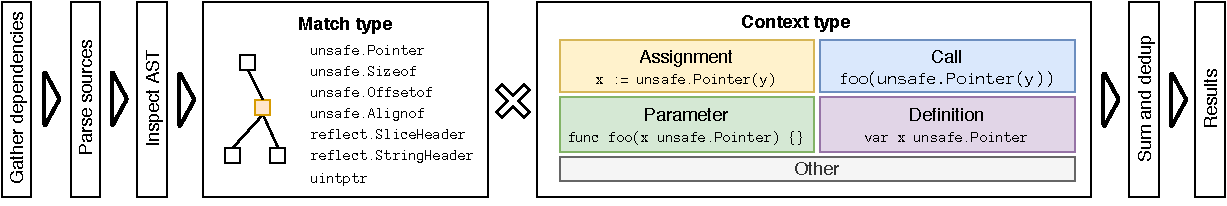
\includegraphics[width=\textwidth]{assets/figures/chapter4/go-geiger-architecture.pdf}
    \caption{Architecture of the \toolGeiger{} tool to detect unsafe usages}
    \label{fig:geiger-architecture}
    %\vspace{-10pt}
\end{figure}


%\subsubsection*{Implementation}

We detect all usages of methods and fields from the \textit{unsafe} package, specifically: \textit{Pointer}, \textit{Sizeof}, \textit{Offsetof}, and \textit{Alignof}.
Furthermore, because they often are used in unsafe operations, we also count occurrences of \textit{SliceHeader} and \textit{StringHeader} from the \textit{reflect} package, and \textit{uintptr}.
All of these usages are referred to as \unsafe{} usages in this paper.
%The first six \unsafe{} types are detected by finding selector expression nodes with matching field names, while \textit{uintptr} usages are found by inspecting identifier nodes in the AST.
Additionally, we determine the context in which the \unsafe{} usage is found, i.e., 
the type of statement that includes the \unsafe{} usage.
In \toolUsage{} we distinguish between assignments (including definitions of composite literals and return statements), calls to functions, function parameter declarations, general variable definitions, or other not further specified usages.
We determine the context by looking up in the AST starting from the node representing the \unsafe{} usage, and identifying the type of the parent node.
%For example, if the nearest relevant ancestor in the AST is an \textit{AssignStmt} node, then the context is determined as assignment.

%% ---------------------------------------------------



